{%\color{red}
\chapter{Performance models}

\section{Code parameters}

\subsection*{Work}

With $W$ we denote work. It is the number of operations executed by a program or algorithm. It could refer to any type of operation, but here we always measure work in floating point operations (FLOPs) in double precision.
We don't count instructions because one instruction can perform more than one floating point operation.

In kernels like dot product, there is often multiplication followed by addition. To make these computations more efficient, many modern CPU architectures compute operations similar to $a=a+b*c$ in one instruction. This type of instructions is called fused multiply-add (FMA).
Other widely used computation is applying the same operation on many operands, vector addition $A[:]=B[:]+C[:]$. This is in hardware implamanted using so called vector instructions. Advanced Vector Extensions (AVX) operates on registers of size 256\,b, which can store 4 operands in double precision or 8 in single precision. One AVX instruction performs 4 FLOPs. And AVX2 adds support of vectorized FMA operations, so 8 FLOPs are performed in a single instruction.

\subsection*{Performance}

Performance refers to number of operations per unit of time.
If program finishes performs $W$ operations and finishes the computations in time $T$, then it achieves performance $P = W/T$.

\subsection*{Memory traffic}

Before processor can perform computations, data has to be loaded to registers. The data has to travel form memory to the L3 cache, then to L2 and L1 and finally to the registers. The registers and cache have very limited size, so after the computations when the data are not needed anymore, it has to travel through the hierarchy back to memory.

We denote the data transfered from memory to L3 cache $Q_r$ (read) and the data transfered from L3 cache to memory $Q_w$ (write), all measured in bytes. The memory traffic is $Q = Q_r + Q_w$.
We could also examine traffic between different cache levels, but for the memory traffic we are interested only in the data transfered between memory and the L3 cache.

\subsection*{Operational intensity and code balance}

The operational intensity is a ratio between work and memory traffic $I = W / Q$, number of floating point operations for 1\,B or memory transfer.
Similar to operational intensity is arithmetic intensity, but it is defined as \todol{todo}.

Sometimes it is more convenient using code balance instead of operational intensity. This is defined as $B_c = I^{-1} = Q / W$, number of bytes per one floating point operation.

\section{Machine parameters}

\subsection*{Peak performance}

Peak performance is theoretical maximum the porcessor is designed to compute. To achieve the peak performance, the processor must utilize all cores and in every cycle it executes the instructions that compute the most operations. Typically these are the AVX (4 FLOPs/cycle) or AVX2 instructions (8 FLOPs/cycle).
As and example let's look at an Intel Xeon E5-2695 v3. This is a 14 core CPU with Haswell architecture and frequency 2.3\.GHz. The Haswell architecture supports AVX2 and can execute two instrucitons per cycle.
So the peak performance is $P_{peak} = 2.3 * 14 * 8 * 2 = 515.2\,\textrm{GFLOPs/s}$.
Evaluation of the peak performance of modern CPUs is not as easy as it seems. It depends on an instruction set and number and type of units in a core. Nice analysis of different Intel architectures can be found in \cite{dolbeau-2018}.

However, the peak performance is a theoretical maximum that most real world applications are not able to achieve.
For example if compiler cannot vectorize the code, the performance drops by factor of four. And if a kernel uses only addition or only multiplication, for example sum of elements in a vector, then the performnace drops to a half.
Instead of peak performance we use attainable performance, denoted as $P_{max}$. This allows more realistic expectations based on knowledge of the code and instructions set used by the compiler.

\subsection*{Memory bandwidth}

Memory bandwidth $b_s$ is a rate at which data can be read and stored into memory.
The bandwidth found in a datasheet does not have to be reachable by the app, similar to the peak performance.
The memory bandwidth depends on access pattern, number of threads, if NUMA is used and Cluster-on-Die\footnote{Cluster-on-Die (CoD) solves a problem with saturation of memory bandwidth on server CPUs from Intel. These CPUs have many cores (14 or more), but only few can are able to saturate the memory bandwidth. When CoD is enabled, the cores, memory and L3 cache are split to two NUMA domains and second memory controller is used. This reduces the number of cores using the same memory controller and doubles the memory bandwidth.} enabled.
More realistic bandwidth can be obtained using micro-benchmark, ideally with similar memory access pattern as the application.

\subsection*{Machine balance}

Machine balance $B_m = b_s / P_{max}$ is a ratio of memory bandwidth and attainable performance.
If $B_c < B_m$ then the code’s performance is limited by the max performance, it is compute bound. Optimizing memory access of such code does not improve performance. One should focus on optimizing computations, for example using vector instructions as much as possible.
If $B_c > B_m$ then the code’s performance is limited by the memory bandwidth, hence it is memory bound. Here performance can be improved by optimizing memory access pattern, for example by reusing data loaded to cache us much as possible, so they don't have to be loaded from memory.

\section{LIKWID tools}

For performance engineering it is essential to get information about hardware (CPU cores and frequency, cache sizes, NUMA topology, \dots). It is also important to have benchmarks that help to better understand important details of given architecture, for example the memory bandwidth.

Linux offers tools that provide information about available hardware and its topology, for example
\begin{lstlisting}
$ cat /proc/cpuinfo
$ cat /proc/meminfo
$ lscpu
$ numactl --hardware
\end{lstlisting}
However these tools are not very user friendly. Reading output of some of these tools, especially \texttt{/proc/cpuinfo} is difficult. And some information, like topology of caches, is not easy to find.

Also writing a benchmark is not as easy as it seems. When writing a benchmark, one wants to measure something specific, which might not be understood by the compiler. Compiler does a lot of optimizations. If results of some computations are not used, these computations are often dropped. Or compiler can replace a code by more efficient implementation, but then the resulting binary does not measure what was intended.

To support performance engineering, a team at University of Erlangen developed a set of tools called LIKWID (Like I Knew What I’m Doing). This suite contains a lot of useful tools for finding information about hardware, measuring performance using hardware counters in a CPU, set of benchmarks and more.
Here is a list of some of the tools:

\begin{itemize}
    \item \texttt{likwid-topology}: print thread, cache and NUMA topology
    \item \texttt{likwid-pin}: pin threaded application (pthread, OpenMP) to dedicated processors
    \item \texttt{likwid-perfctr}: configure and read out hardware performance counters
    \item \texttt{likwid-bench}: Micro benchmarking platform
\end{itemize}

\section{Roofline model}

The Roofline model brings together two machine parameters describing possible bottlenecks, maximum performance $P_{max}$ and memory bandwidth $b_s$, and visualizes upper bound of performance any code can achieve on given machine.
It is a graph with operational intensity $I$ on the x-axis and performance $P$ on the y-axis. The two bottlenecks are displayed as two lines:
The horizontal line is a visualizaiton of attainable performance $P = P_{max}$.
The skewed line is a function of memory bandwidth and operational intensity $P = I * P_{max}$.
As these are the factors limiting the performance, we can expect performance of any program must be below these lines or in the best case on the lower of the two limits.
We can write the performance upper bound as a function of either operational intensity or code balance as
\begin{equation}
   P = min(P_{max}, I \cdot b_s) = min(P_{max}, b_s / B_c).
\end{equation}
This can be visualized as \todol{ref naive graph}.
The shape of the graph is what gives the model its name.

Any compute kernel can be shown in the graph as a vertical line under the roofline. X-coordinate of the line is the operational intensity of the kernel.
We can expect the performance of given kernel is somewhere along this line. Closer to the roofline (higher) is better, but the it can never exceed the roofline.

The point where the two lines intersect is at operational intensity $I = B_m^{-1}$. At this point the performance $P_{max}$ is achieved while reading and writing to memory as much as possible, $b_s$\,B/s.
Performance of any kernel on the right side of this point ($B_c < B_m$ or $I > B_m^{-1}$) is limited by $P_{max}$. We call such kernel compute bound.
Performance of any kernel on the left side of this point ($B_c > B_m$ or $I < B_m^{-1}$) is limited by $b_s$. We call such kernel memory bound.

%\todop{
%\begin{itemize}
%    \item naive, ceilings
%    \item cite williams
%\end{itemize}
%}

\begin{figure}[H]
   \centering
   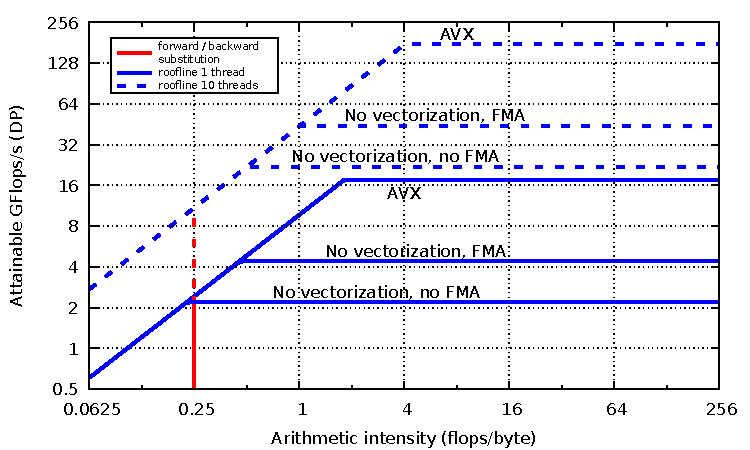
\includegraphics[width=0.7\textwidth,clip=true]{images/roofline_emmy_Xeon2660v2}
   \caption{Roofline model of the  Intel Xeon E5-2660 v2 CPU.}
  \label{fig:roofline_emmy}
\end{figure}


%\todop{
%\begin{itemize}
%    \item Description of CPU
%    \item Memory hierarchy
%\end{itemize}
%}






\section{ECM -- DAXPY}
\label{sec:epm}

The Roofline model~\cite{williams-2009} is a simple model
for performance prediction in the saturated case.
Hereby it is assumed code is limited by floating-point performance or by the
memory bandwidth.

The ECM performance model~\cite{treibig-2010-ecm,hager-2012-ecm} is a refinement
of Roofline model. 
In contrast it allows a performance prediction on the single core level as well
as a scaling prediction over the socket.
The model takes into account the duration of the code execution inside the core
separated by arithmetic and data movement.
Furthermore data transfers in the memory/cache hierarchy are considered as well
as the achievable memory bandwidth.
%
Finally both parts build the single core model, which is used to determine the
scaling behaviour over the cores until a bottleneck is reached. 
%
For memory bound codes this is typically the achievable memory bandwidth as all
other infrastructure like Intel's L3 cache on Ivy Bridge, Haswell, and Broadwell
scales perfectly. 

The ECM model has some restrictions on the code to be analysed.
It is important that streaming accesses are performed. This means prefetching
works perfectly and can hide latency effects.

In the following text we give a brief introduction to the model by analyzing a
simple daxpy like kernel on the HSW-S system, which's processor is based on the Intel Haswell
microarchitecture. For further details regarding the ECM model refer
to~\cite{stengel-2015}.  The daxpy kernel to be analysed is:
%
\begin{lstlisting}
for (int i = 0; i < N; ++i) 
  r[i] +=  s * l[i];
\end{lstlisting}
%
The vectors \verb'r' and \verb'l' are double-precision floating point vectors
with \verb'N' elements each. 
The \verb'index' vector consists of $4$\,B integers.
Furthermore \verb's' is a scalar double precision floating point variable.
%
The code is vectorized via AVX and FMA3 instructions by the compiler and
additionally $4$-way unrolled to reach full performance.
%Effectively one iteration of the compiler
%generated loop performs $16$ iterations of the original kernel.
%
For easier modeling we take so many iterations into account, which are needed to
process a whole cache line.
Hence, for the daxpy kernel with double precision floating point numbers our
work package we model is eight iterations.
%
To process these eight iterations with AVX and FMA3 four $32$\,B AVX loads (\verb|r[:]| and
\verb|l[:]|), two
$32$\,B AVX stores (\verb'r[:]'), and two fused-multiply-adds are required.
%
Hereby we define the ``work'' performed by eight iterations is to transfer $W = 192$\,B.
%
In order to determine the duration of the execution of the code inside
the core we assume all operands reside in L1 cache.

\begin{figure}[tp]
  \centering
  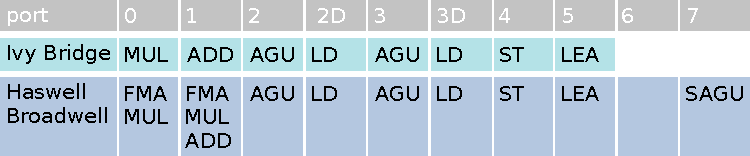
\includegraphics[width=0.49\textwidth,clip=true]{images/IntelMicroArchPorts}
  \caption{Ports and associated execution units of Intel microarchitectures.
Only the units relevant for this paper are shown.}
  \label{fig:ports}
\end{figure}

\begin{figure}[tp]
  \centering
  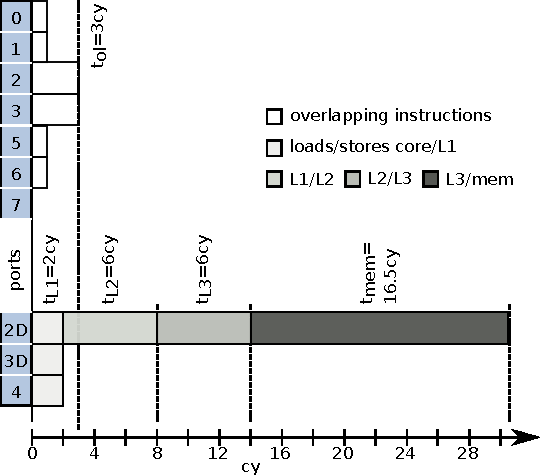
\includegraphics[width=0.42\textwidth,clip=true]{images/ecm-hsw-daxpy}
  \caption{Run time contributions of different execution ports and cache/memory
hierarchy levels for eight iterations of the daxpy kernel on HSW-S (Haswell micro
architecture). In contrast to the IACA prediction instructions on port~$7$
(hashed) seem to be executed on ports~$2$ and~$3$ (hashed).}
  \label{fig:daxpy:ecm}
\end{figure}

\begin{figure}[tp]
  \centering
  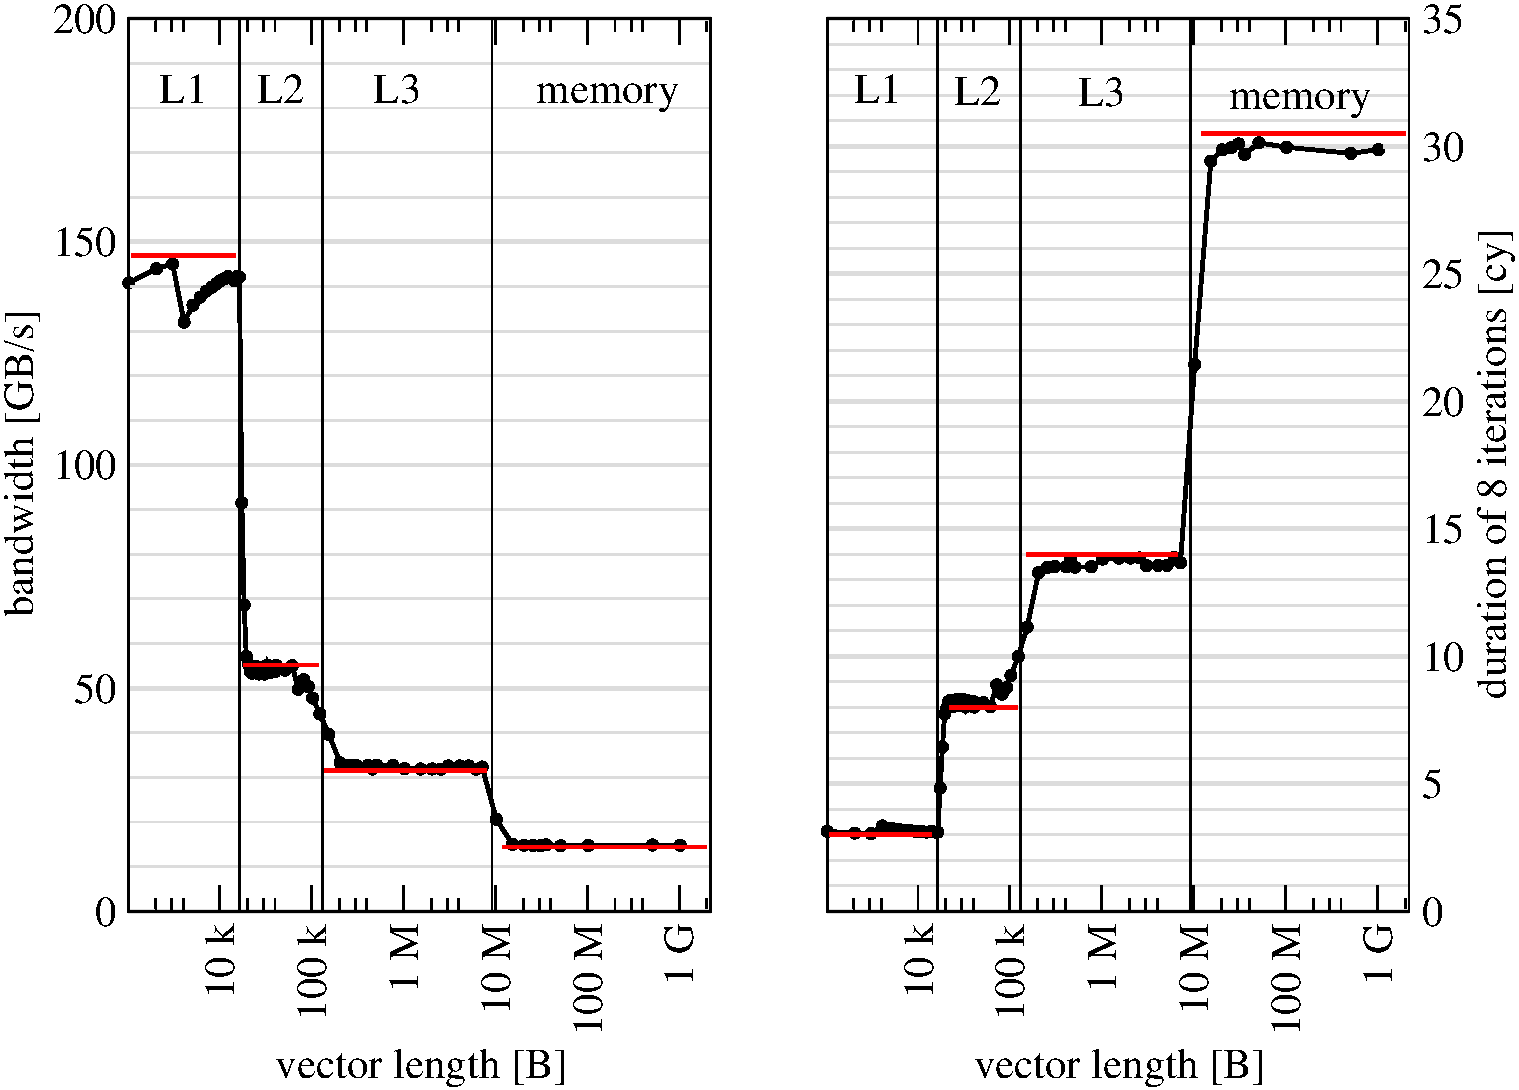
\includegraphics[width=0.49\textwidth,clip=true]{images/daxpy-bw-hasep1-f-2.3-w-cy}
  \caption{Bandwidth and duration of 16 iterations, i.\,e.\ one iteration of the
compiler generated loop, for the daxpy kernel on HSW-S. Note that the total
working set required for vectors
\protect\texttt{r} and \texttt{l} is twice the vector length.}
  \label{fig:daxpy:perf}
\end{figure}

The duration of the incore execution depends on the core's architecture.
For HSW-S it's the Haswell micro architecture.
The super-scalar design has several ports with different execution units for
different types of instructions, shown as part of Fig.~\ref{fig:ports}.
Instructions scheduled to different ports run independently.
The instruction scheduler takes care that no data dependencies are violated.
Instructions inside ports are pipelined, but only one instruction per port can
be issued per cycle.
Haswell can perform two loads (LD, port~$2D$ and~$3D$) and one store (ST,
port~$4$) of sizes up to $32$\,B at the same time~\cite{intel-orm-2016}, each.
Each load and store requires an address to be generated by an address
generation unit (AGU, port~$2$,~$3$, and~$7$).
However on port~$7$ only a simple AGU is located, which is limited to simple
addressing modes~\cite{intel-orm-2016,hofmann-2016-hsw}.
%
For floating point operations relevant, the cores hosts two fused multiply add
(FMA) units (port~$0$ and~$1$), two multiplication (MUL) units (port~$0$
and~$1$), and one add (ADD) unit (port~$1$).

We could manually analyse the assembly code of the daxpy kernel and create a
scheduling of the instructions onto the ports to determine the duration of the
execution inside the core.
This is not feasible for complex kernels and requires often internal knowledge
of the core, which is publicly not available.
Instead we use Intel's Architecture Code Analyzer~\cite{intel-iaca} (IACA)
for this task. 
We use the tool's throughput mode, were it is assumed, that iterations of the
loop are independent and can overlap due to the out-of-order engine.
Further we assume no pipeline bubbles of the different ports. 
The distribution of the instructions over the ports is found in
Fig.~\ref{fig:daxpy:ecm}.
For the ECM model the duration of the execution inside the core is split into
two categories.
The first one comprises only data movement between registers and L1 cache,
i.\,e.\ loads and stores occurring on port~$2D$,~$3D$, and~$4$.
The second category consists of the rest, which can possibly overlap with the
loads and stores, like arithmetic, logic, and address generation.
%
From the IACA analysis we get 
\be
  t_\text{ol} = 2\,\cyw
\ee
%
(normalized to eight iterations) as the maximum duration on the ports \textit{overlapping} overlapping with data
movements.
The maximum duration on the latter ports $t_\text{L1}$, is
\be
  t_\text{L1} = 2\,\cyw.
\ee
%
Note that the compiler uses simple addressing for store addresses, which
according to IACA will utilize the simple AGU on port~$7$.
%
%
The performance $P_\text{L1}$, when all data is fetched from L1, is then
computed as 
%
\be
  P_\text{L1} = \frac{W}{\max(t_\text{ol}, t_\text{L1})} f,
\ee
%
where $W$ denotes the loop specific work performed and $f$ clock
frequency of the core.
For this loop with $W=192$\,B and $f=2.3$\,GHz we have $P_\text{L1} =
220.8$\,GB/s. 
Measurements shown in Fig.~\ref{fig:daxpy:perf} reveal that only around
$145$\,GB/s are reached.
It seems that the SAGU on port~$7$ is not used, causing the store addresses to
be generated by the two remaining AGUs.
This causes $t_\text{ol}$ to be increased by $1$\,\cyw and becoming the new
bottleneck.
This results in a corrected
%
\be
   t_\text{ol} = 3\,\cyw
\ee
%
with $P_\text{L1} = 147.9$\,GB/s, which is in line with the measurements.


Modeling the performance when data resides in different cache levels from L1
requires analysing data transfers between these levels.
For daxpy this is straight forward as vector \verb'r' and \verb'l' are
streamed from/to memory and no cache reuse takes place.
Throughout the cache/memory hierarchy we transfer between each cache level three 
cache lines (cl) for each iteration: load $1$\,cl of \verb'l', load $1$\,cl of
\verb'r', and store $1$\,cl of \verb'r'.

Transferring a cache line between L1/L2 and L2/L3 takes $2$\,cy each.
Hence it takes
%
\be
  t_\text{L2} = 6\,\text{cy} \qquad \text{and} \qquad t_\text{L3} = 6\,\text{cy}
\ee
%
to transfer our three cache lines, respectively.
For computing the performance $P_\text{L2}$ and $P_\text{L3}$, when data resides
in L2 or L3 cache, respectively, we have to add $t_\text{L2}$ and $t_\text{L3}$
to the duration of the data path, as on the considered Intel architectures data
transfers seem be be serialized when streaming accesses occur\footnote{This need
not to be the actual implementation inside the architecture, it only resembles
the observation and can be different on other architectures.}.
The performance is then
%
\begin{align}
  P_\text{L2} &= \frac{W}{\max(t_\text{ol}, t_\text{L1} + t_\text{L2})} f, \\
  P_\text{L3} &= \frac{W}{\max(t_\text{ol}, t_\text{L1} + t_\text{L2} +
t_\text{L3})} f.
\end{align}
%
In our case $P_\text{L2} = 55.2$\,GB/s and $P_\text{L3} = 31.5$\,GB/s.
%

How many cache lines per cycle can be transferred between L3 and memory could
theoretically be obtained by taking the nominal memory bandwidth into account.
However, this bandwidth is practically never reached and depends strongly on the
access pattern used.
This is caused by the organization of the memory subsystem, where e.\,g.\ banking
conflicts and DRAM page misses incur performance.
With detailed knowledge about the internals of the (closed IP) memory controller
(scheduling strategies, thresholds for strategy switching, ...) and DRAM modules
this could also be modeled, which is far from being trivial~\cite{jacob-2007}.
As this is beyond the scope of the ECM model typically a micro benchmark
resembling the used access pattern by the code under investigation is used
to measure the attainable bandwidth and use it as input for the model.
%
For this model we use \textsc{McCalpin's} STREAM copy
benchmark~\cite{mccalpin-1995} which achieves (without nontemporal stores and
including the write allocate) a bandwidth of $\approx 26.9$\,GB/s when all seven cores
of a cluster are utilized.
With the core's clock frequency of $2.3$\,GHz it takes $5.5$\,cy to transfer one
cache line between L3 cache and memory.
Transferring our three cache lines between these to levels takes then
%
\be
  t_\text{mem} = 16.5\,\text{cy}.
\ee
%
The performance $P_\text{mem}$, when every vector is streamed from memory, is then
%
\be
  P_\text{mem} = \frac{W}{\max(t_\text{ol}, t_\text{L1} + t_\text{L2} +
t_\text{L3} + t_\text{mem})} f.
\ee
%
This leads to $P_\text{mem} = 14.5$\,GB/s. 

\section{ECM -- Indirect DAXPY}

%
\begin{lstlisting}
for (int i = 0; i < N; ++i) 
  r[idx[i]] +=  s * l[i];
\end{lstlisting}
%
which resembles an indirect addressed daxpy.
The vectors \verb'r' and
\verb'l' are double-precision floating point vectors with \verb'N' elements
each. 
The \verb'idx' vector contains $4$~B integers.
Furthermore \verb's' is a scalar double precision floating point variable.
%
The code is 4-way unrolled and by the compiler, when
optimizations are turned on and target ISA is AVX2 and FMA3. One iteration
over this newly formed loop now performs 4 scalar iterations. The code snipped
from above effectively becomes:
%
\begin{lstlisting}
for (int i = 0; i < N; i += 4) {
  r[idx[i    ]] += s * l[i    ];
  r[idx[i + 1]] += s * l[i + 1];
  r[idx[i + 2]] += s * l[i + 2];
  r[idx[i + 3]] += s * l[i + 3];
}
\end{lstlisting}
%
For the ECM model we determine the duration of the execution of the code inside
the core under the assumption all operands reside in L1 cache.

\begin{figure}[tp]
  \centering
  \includegraphics[width=0.49\textwidth,clip=true]{images/ecm-hsw-daxpy-indirect}
  \caption{xxx}
  \label{fig:xxx}
\end{figure}

\begin{figure}[tp]
  \centering
  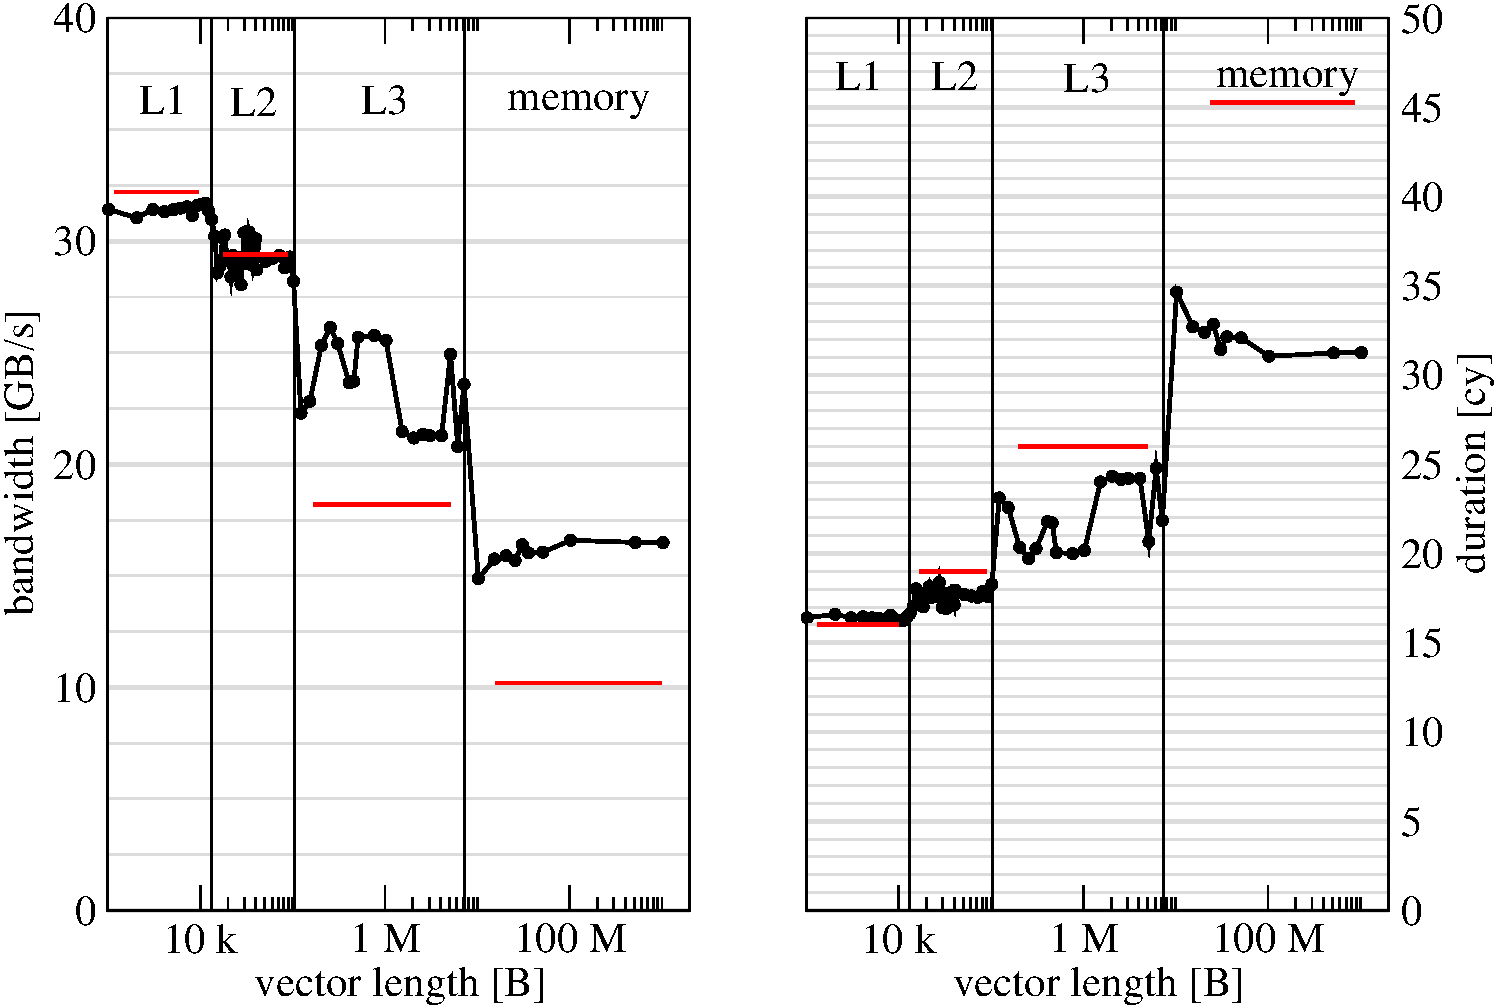
\includegraphics[width=0.49\textwidth,clip=true]{images/daxpy-indirect-bw-hasep1-f-2.3-w-cy}
  \caption{xxx}
  \label{fig:daxpy-indirect:perf}
\end{figure}

The complied loop requires eight $8$\,B loads (\verb|r[:]| and
\verb|l[:]|), four $4$\,B loads (\verb'idx[:]'), four
$8$\,B stores (\verb'r[:]'), and $16$ address generations.
Furthermore four scalar fused-multiply-adds are used. 
\todo{Instructions regarding loop and index counter increments as well as address
computations are for this case negligible.}
We define performed by one iteration of the compiler created loop to be $W =
112$\,B.

How long the execution takes depends on the underlying architecture. 
In order to determine this, we take a look at the Intel Haswell
microarchitecture in Fig.~\ref{fig:ports}.
The super-scalar design has several ports with different execution units for
different types of instructions.
Instructions scheduled to different ports run independently.
The instruction scheduler takes care that no data dependencies are violated.
Instructions inside ports are pipelined, but only one instruction per port can
be issued per cycle.
Haswell can perform two loads (port $2D$ and $3D$) and one store (port $5$) of
sizes up to $32$\,B at the same time~\cite{agner-2016-11-3}, each.
This constellation requires the store address to be simple addressing as only in
this case the address generation unit (AGU) on port~$7$ can be used.
\todo{What means simple addressing?, cite Hofmann}. 
% Effectively this boils down to either two loads or one load and store.
%
For floating point operations relevant, it hosts two FMA units (port 0 and
1) two MUL units (port 0 and 1), and one ADD unit (port 1).
\todo{describe lea}

Under this considerations one iteration of the compiled loop would require $2$\,cy
for the FMA (port $0$ and $1$), $6$\,cy for the twelve loads (port $3$ and $4$),
and $4$\,cy for the four stores (port $5$).
From the $16$ address generation two are simple an can run on the simple AGU on
port $7$ requiring $2$\,cy, whereas the remaining $14$ addresses are handled in
$7$\,cy due to two AGUs on port $3$ and $4$.
We assume that the out-of-order engine can fill bubbles in the pipelines of the
different ports as the loop iterations are independent of each other.
We classify the ports into arithmetic/logic (port $0$, $1$, $5$, and $6$) and
data movement (port $2$, $3$, $4$, and $7$). 
The maximum duration $t_\text{ol}$ of the first class of ports is 
%
\be
  t_\text{ol} = \max(2\,\cyw, 2\,\cyw, 3\,\cyw, 3\,\cyw)
= 3\,\cyw
\ee
%
and the maximum duration of the data movement ports $t_\text{L1}$ which
load/store data from/to L1 is
\be
  t_\text{L1} = \max(6\,\cyw, 7\,\cyw, 4\,\cyw, 2\,\cyw) =
7\,\cyw.
\ee
%
% for the duration of the data transfers between core and L1 cache.
%
The performance $P_\text{L1}$, when all data is fetched from L1, is then computed as 
%
\be
  P_\text{L1} = \frac{W}{\max(t_\text{ol}, t_\text{L1})} f,
\ee
%
where $W$ denotes the loop specific work performed and $f$ clock frequency of the core.
For this loop with $W=112$\,B and $f=2.3$\,GHz we have $P_\text{L1} =
36.8$\,GB/s. On HSW1 only $\approx 31$\,GB/s, i.\,e.\ 80\,\% of the predicted
performance are achieved for this loop, shown in Fig.~\ref{fig:daxpy-indirect:perf}.

Modeling the performance when data resides in different cache levels from L1
requires to analyse the data transfers between these levels.
In this case this is straight forward as vector \verb'r', \verb'l', and
\verb'idx' are streamed from/to memory and no cache reuse takes place.
Throughout the cache/memory hierarchy we transfer between each cache level
$112$\,B $= 1.75$\,cl (cache lines) for each iteration: load $32$\,B of
\verb'l', load $32$\,B of \verb'r', load $16$\,B of \verb'idx' and store $32$\,B
of \verb'r'.

Transferring a cache line between L1/L2 and L2/L3 takes $1$\,cy and $2$\,cy,
respectively. Hence it takes
%
\be
  t_\text{L2} = 1.75\,\cyw \text{and} t_\text{L3} = 3.5\,\cyw
\ee
%
to transfer our $112$\,B.
For computing the performance $P_\text{L2}$ and $P_\text{L3}$, when data resides
in L2 or L3 cache, respectively, we
have to add $t_\text{L2}$ and $t_\text{L3}$ to the duration of the data path, as on the considered
Intel architectures data transfers seem be be serialized when streaming accesses
occur\footnote{This need not to be the actual implementation inside the
architecture, it only resembles the observation and can be different on other
architectures.}.
The performance is then
%
\begin{align}
  P_\text{L2} &= \frac{W}{\max(t_\text{ol}, t_\text{L1} + t_\text{L2})} f, \\
  P_\text{L3} &= \frac{W}{\max(t_\text{ol}, t_\text{L1} + t_\text{L2} +
t_\text{L3})} f.
\end{align}
%
In our case $P_\text{L2} = 29.4$\,GB/s and $P_\text{L3} = 18.2$\,GB/s.
%

How many cache lines per cycle can be transferred between L3 and memory could
theoretically be obtained by taking the nominal memory bandwidth into account.
However, this bandwidth is practically never reached and depends strongly on the
access pattern used.
This is caused by the organization of the memory subsystem, where e.\,g.\ banking
conflicts and DRAM page misses incur performance.
With detailed knowledge about the internals of the (closed IP) memory controller
(scheduling strategies, thresholds for strategy switching, ...) and DRAM modules
this could also be modeled, which is far from being trivial~\cite{jacob-2007}.
As this is beyond the scope of the ECM model typically a micro benchmark
resembling the used access pattern by the code under investigation is used
to measure the attainable bandwidth and use it as input for the model.
%
For this model we use \textsc{McCalpin's} STREAM copy
benchmark~\cite{mccalpin-1995} which achieves (without nontemporal stores and
including the write allocate) a bandwidth of $\approx 26.9$\,GB/s when all seven cores
of a cluster are utilized.
With the core's clock frequency of $2.3$\,GHz it takes $5.5$\,cy to transfer one
cache line between L3 cache and memory.
Transferring our $112$\,B between these to levels takes
%
\be
  t_\text{mem} = 9.625\,\cyw.
\ee
%
The performance $P_\text{mem}$, when every vector is streamed from memory, is then
%
\be
  P_\text{mem} = \frac{W}{\max(t_\text{ol}, t_\text{L1} + t_\text{L2} +
t_\text{L3} + t_\text{mem})} f.
\ee
%
This leads to $P_\text{mem} = 10.2$\,GB/s. 

% The required information on the hardware capabilities can be obtained from the
% data sheets of the vendors or measured via micro-benchmarks.
% For good estimates regarding achievable memory bandwidth a benchmark which
% exhibits the same access pattern as the code under investigation is preferable.
% %
% In our case primarily the nonzeros from matrix $L$ out of the \vlnz{}
% array are loaded from memory.
% Hereby we neglect, that for each panel also the indices into the right hand side
% $r$ must be loaded. 
% This seems to be a fair assumption for matrices with large panel sizes, like the
% dense\footnote{MW: here already reference to the dense matrix} matrix with $n_p = 80$.
% Here only for the panel's first column, indices must be loaded from memory
% and can be $79$ times reused.
% Further we ignore that during forward substitution stores to $r$ occur.
% %
% The most simple benchmark, which resembles this behavior, is linearly reading
% from memory.
% We accomplish this by summing up the elements of a vector $a$ which is large
% enough to reside in memory: \texttt{s = s + a[i]}.
% Note that the single core bandwidth for read only is below the STREAM copy
% bandwidth (\texttt{a[i] = b[i]}).
% Here \textsc{McCalpin} identifies limited concurrency as the
% bottleneck\footnote{Comment of \textsc{McCalpin} in the Intel Forum found under
% \texttt{http://software.intel.com/en-us/forums/topic/456184}.}.
% However in the saturated case a higher bandwidth compared to STREAM copy is
% achieved.
% Through an $n$-way unrolling over columns
% (described in section~\ref{sec:pm:dt:wu}) there are effectively $n$ concurrent
% read streams for each core.
% For simplicity we ignore the fact that with $n > 1$ possibly the attainable
% bandwidth decreases.
% %
% Table~\ref{tab:hw} contains all the ECM model parameters used for the different
% hardware systems.
% 


}